%%%%%%%%%%%%%%%%%%%%%%%%%%%%%%%%%%%%%%%%%%%%%%%%%%%%%%%%%%%%%%%%%%%%%%%%%%%%%%
%
% Section file included in main project file using \input{}
%
% Assumes that LaTeX2e macros and packages defined in cg_comp.sty are
%   available
%
%%%%%%%%%%%%%%%%%%%%%%%%%%%%%%%%%%%%%%%%%%%%%%%%%%%%%%%%%%%%%%%%%%%%%%%%%%%%%%

 \section{Simple Model of Guitar Intonation\label{sct:model}}

Fundamental frequency of a string~\cite{ref:morse1981vas,ref:morse1981vsa}:
 \begin{equation} \label{eqn:f_0_def}
f_0 = \frac{1}{2\, L_0}\, \sqrt{\frac{T_0}{\mu_0}}\, ,
 \end{equation}
where $L_0$ is the length of the free (unfretted) string from the saddle to the nut, $T_0$ is the tension in the free string, and $\mu_0 \equiv M / L_0$ is the linear mass density of a free string of mass $M$.

 \begin{equation} \label{eqn:f_0_stiff}
f_0 = \frac{1}{2\, L_0}\, \sqrt{\frac{T_0}{\mu_0}} \left[ 1 + B_0 + \left(1 + \frac{\pi^2}{8}\right) B_0^2 \right]\, ,
 \end{equation}
where $B_0$ is a ``string stiffness parameter.'' For a uniform string with a cylindrical cross section, $B_0$ given by~\cite{ref:morse1981vsb}
 \begin{equation} \label{eqn:b_def}
B_0 \equiv \sqrt{\frac{\pi\, R^4 E}{T_0\, L_0^2}}\, ,
 \end{equation}
where $R$ is the radius of the string and $E$ is Young's modulus (or the modulus of elasticity). For a typical nylon guitar string with $E \approx 2 - 4$~GPa, $T_0 \approx 50 - 70$~N, $R \approx 0.35 - 0.51$~mm, and $L_0 \approx 650$~mm, we have $B_0 \approx 0.007 - 0.026$, indicating that the corrections in \eqn{f_0_stiff} are not significant.

Throughout this work, we will use \emph{cents} to describe small differences in pitch~\cite{ref:durfee2015pms}. One cent is one one-hundredth of a 12-TET half step, so that there are 1200~cents per octave. The difference in pitch between frequencies $f_1$ and $f_2$ is therefore defined as
 \begin{equation} \label{eqn:cents_def}
\Delta \nu \equiv 1200\, \log_2\left(\frac{f_2}{f_1}\right)\, .
 \end{equation}
We define $f \equiv (f_1 + f_2) / 2$ and $\Delta f \equiv f_2 - f_1$. Then
 \begin{equation} \label{eqn:cents_approx}
\Delta \nu = 1200\, \log_2\left(\frac{f + \Delta f / 2}{f - \Delta f /2}\right) \approx \frac{1200}{\ln 2}\, \frac{\Delta f}{f}\, ,
 \end{equation}
where the last approximation applies when $\Delta f \ll f$. An experienced guitar player can distinguish beat notes with a difference frequency of $\Delta f \approx 1$~Hz, which corresponds to 8~cents at $A_2$ ($f = 220$~Hz) or 5~cents at $E_4$ ($f = 329.63$~Hz).

 \begin{figure}
  \centering
  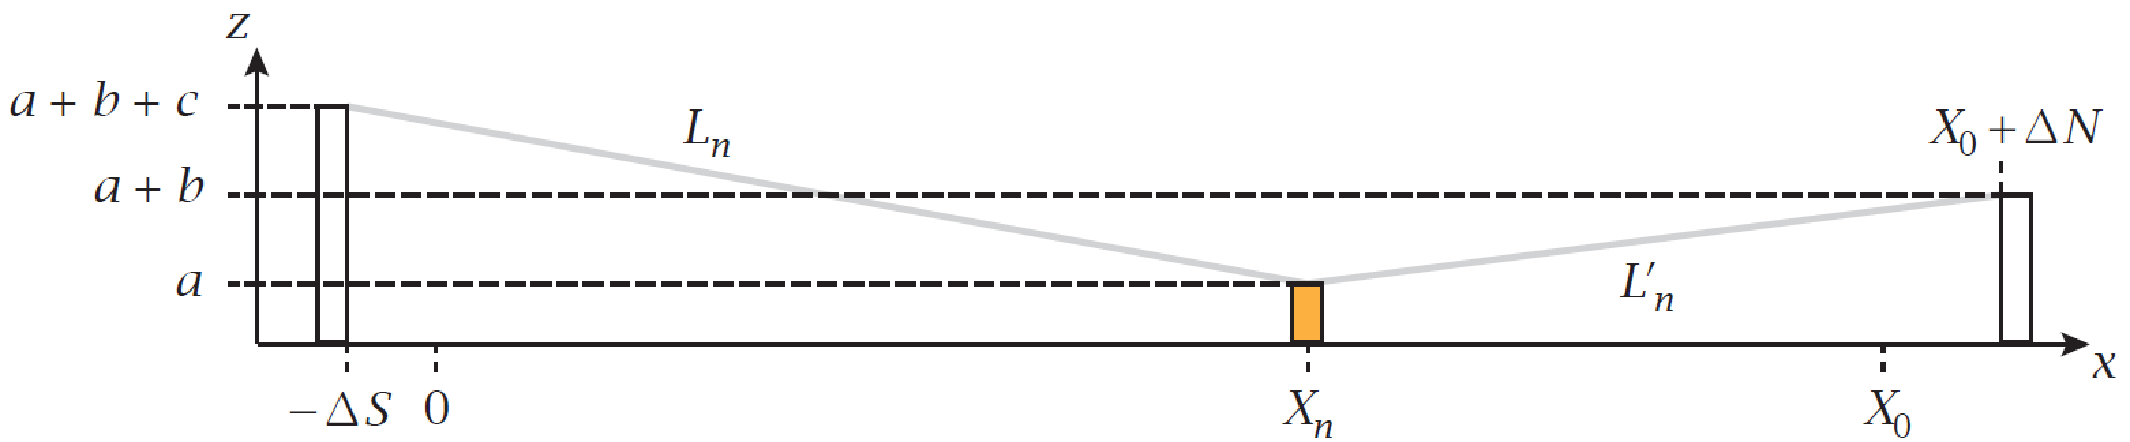
\includegraphics[width=6.0in]{figures/guitar_schematic}
  \caption{\label{fig:guitar_schematic} A simple (side-view) schematic of the classical guitar used in this model. The scale length of the guitar is $X_0$, but we allow the edges of both the saddle and the nut to be set back an additional distance $\Delta S$ and $\Delta N$, respectively. The location on the $x$-axis of the center of the $n^\textrm{th}$ fret is $X_n$. In the $z$ direction, $z = 0$ is taken as the surface of the fingerboard; therefore the height of each fret above the fingerboard is $a$, the height of the nut is $a + b$, and the height of the saddle is $a + b + c$. $L_n$ is the \emph{resonant length} of the string from the saddle to the center of fret $n$, and $L^\prime_n$ is the length of the string from the fret to the nut.}
 \end{figure}

Our model begins with the schematic of the guitar shown in \fig{guitar_schematic}. The scale length of the guitar is $X_0$, but we allow the edges of both the saddle and the nut to be set back an additional distance $\Delta S$ and $\Delta N$, respectively. The location on the $x$-axis of the center of the $n^\textrm{th}$ fret is $X_n$. In the $z$ direction, $z = 0$ is taken as the surface of the fingerboard; the height of each fret is $a$, the height of the nut is $a + b$, and the height of the saddle is $a + b + c$. $L_n$ is the \emph{resonant length} of the string from the saddle to the center of fret $n$, and $L^\prime_n$ is the length of the string from the fret to the nut. The total length of the string is defined as $\mathcal{L}_n \equiv L_n + L^\prime_n$. For reasons discussed below, we have not adopted a more complicated fretting model~\cite{ref:byers1996cgi,ref:varieschi2010icf}. We start with the simple form of the fundamental frequency of a string given by \eqn{f_0_def}, and apply it to the frequency of a string pressed just behind the $n^\mathrm{th}$ fret:
 \begin{equation} \label{eqn:f_n_def}
f_n = \frac{1}{2\, L_n}\, \sqrt{\frac{T_n}{\mu_n}}\, ,
 \end{equation}
where $T_n$ and $\mu_n$ are respectively the tension and linear mass density of the fretted string. We note that $T_n$ and $\mu_n$ depend on $\mathcal{L}_n$, the \emph{total} length of the fretted string from the saddle to the nut. Ideally, in the 12-TET equal-temperament system~\cite{ref:durfee2015pms},
 \begin{equation} \label{eqn:f_n_tet}
f_n = \gamma_n\, f_0\, , \qquad \textrm{(12-TET~ideal)}
 \end{equation}
where
 \begin{equation} \label{eqn:gamme_n_def}
\gamma_n \equiv 2^{n / 12}\, .
 \end{equation}
Therefore, the error interval expressed in cents is given by
 \begin{equation}\label{eqn:error_def}
 \begin{split}
\Delta \nu_n &= 1200\, \log_2\left( \frac{f_n}{\gamma_n\, f_0} \right) \\
&= 1200\, \log_2 \left( \frac{L_0}{\gamma_n\, L_n}\, \sqrt{\frac{\mu_0}{\mu_n}\, \frac{T_n}{T_0}}\, \right) \\
&= 1200\, \log_2 \left( \frac{L_0}{\gamma_n\, L_n} \right) + 600\, \log_2 \left(  \frac{\mu_0}{\mu_n} \right) + 600\, \log_2 \left( \frac{T_n}{T_0} \right)\, .
 \end{split}
 \end{equation}

The final form of \eqn{error_def} makes it clear that --- for nylon guitar strings --- there are three contributions to intonation:
 \begin{enumerate}
  \item
   \emph{Resonant Length}: The first term represents the error caused by the increase in the length of the fretted string $L_n$ compared to the ideal length $X_n$, which would be obtained if $b = c = 0$ and $\Delta S = \Delta N = 0$.
  \item
   \emph{Linear Mass Density}: The second term is the error caused by the reduction of the linear mass density of the fretted string. This effect will depend on the \emph{total} length of the string, given by $\mathcal{L}_n = L_n + L^\prime_n$.
  \item
   \emph{Tension}: The third (and most complex) term is the error caused by the \emph{increase} of the tension in the string caused by the stress and strain applied to the string by fretting. This effect will also depend on the total length of the string $\mathcal{L}_n$.
 \end{enumerate}
We will discuss each of these three sources of error in turn below.

 \subsection{Resonant Length Error}
We can estimate the first term in the last line of \eqn{error_def} by referring to \fig{guitar_schematic} and computing the resonant length $L_n$. We find:
 \begin{equation}  \label{eqn:l_n_def}
L_n = \begin{cases}
\sqrt{\left(X_0 + \Delta S + \Delta N\right)^2 + c^2}\, , & n =  0 \\
\sqrt{\left(X_n + \Delta S\right)^2 + (b + c)^2}\, . & n \ge 1
 \end{cases}
 \end{equation}
When $b + c \ll X_0$, we can approximate $L_n$ by
 \begin{equation} \label{eqn:l_n_approx}
L_n \approx \begin{cases}
X_0 + \Delta S + \Delta N + c^2/2\, X_0 & n =  0\, , \\
X_n + \Delta S + (b + c)^2/2\, X_n & n \ge 1\, .
 \end{cases}
 \end{equation}
Then --- when the guitar has been manufactured such that $X_n = X_0 / \gamma_n$ --- the resonant length error is approximately
  \begin{equation} \label{eqn:rle_approx}
  1200\, \log_2 \left( \frac{L_0}{\gamma_n\, L_n} \right) \approx -\frac{1200}{\ln(2)} \left[ \frac{\left(\gamma_n - 1\right) \Delta S - \Delta N}{X_0} + \frac{\gamma_n^2 (b + c)^2 - c^2}{2\, X_0^2}\right]
  \end{equation}
If the guitar is uncompensated, so that $\Delta S = \Delta N = 0$, this error is typically less than 0.25~cents. But, with $\Delta S > 0$ and $\Delta N < 0$, we can significantly \emph{increase} the magnitude of this ``error'' and cause the frequency to shift lower. We'll see that this is our primary method of compensation. \red{TBD: Add a figure here?}

Previous studies of guitar intonation and compensation have chosen to include the apparent increase in length of the string caused by both the fretting depth and the shape of the fretted string under the finger~\cite{ref:byers1996cgi,ref:varieschi2010icf}. As the string is initially pressed to the fret, the total length $\mathcal{L}_n$ increases and causes the tension in the string --- which is clamped at the saddle and the nut --- to increase. As the string is pressed further, does the additional deformation of the string increase its tension (throughout the resonant length $L_n$)? There are at least two purely empirical reasons to doubt this hypothesis. First, we can mark a string (with a fine-point felt pen) above a particular fret and then observe the mark with a magnifying glass. As the string is pressed all the way to the finger board, the mark does not move perceptibly --- it has become effectively \emph{clamped} on the fret. Second, we can use either our ears or a simple tool to measure frequencies~\cite{ref:pgtweb} to listen for a shift as we use different fingers and vary the fretted depth of a string. The apparent modulation is far less than would be obtained by classical vibrato ($\pm15$~cents), so we assume that once the string is minimally fretted the length(s) can be regarded as fixed. (If this were not the case, then fretting by different people or with different fingers, at a single string or with a barre, would cause additional, varying frequency shifts that would be audible and difficult to compensate.)

 \subsection{Linear Mass Density Error}
As discussed above, the linear mass density $\mu_0$ of an open (unfretted) string is simply the total mass $M$ of the string clamped between the saddle and the nut divided by the length $L_0$. Similarly, the mass density $\mu_n$ of a string held onto fret $N$ is $M/\mathcal{L}_n$. Therefore
 \begin{equation}
\frac{\mu_0}{\mu_n} = \frac{\mathcal{L}_n}{L_0} \equiv 1 + Q_n\, ,
 \end{equation}
where we have followed Byers and defined~\cite{ref:byers1996cgi,ref:varieschi2010icf}
 \begin{equation} \label{eqn:lambda_n_def}
Q_n \equiv \frac{\mathcal{L}_n - L_0}{L_0}\, .
 \end{equation}
Since we expect that $Q_n \ll 1$, we can approximate the second term in the final line of \eqn{error_def} as
 \begin{equation} \label{eqn:lmd_error}
600\, \log_2 \left(  \frac{\mu_0}{\mu_n} \right) \approx \frac{600}{\ln(2)}\, Q_n\, .
 \end{equation}

Referring to \fig{guitar_schematic}, we see that $\mathcal{L}_n = L_n + L^\prime_n$, and we calculate $L^\prime_n$ as
 \begin{equation}
L^\prime_n = \begin{cases}
0\, , & n =  0 \\
\sqrt{\left(X_0 - X_n + \Delta N\right)^2 + b^2}\, . & n \ge 1
 \end{cases}
 \end{equation}
Assuming that $b^2 \ll X_0 - X_n$, we expand the $n \ne 1$ expression to obtain
 \begin{equation}
L^\prime_n \approx X_0 - X_n + \Delta N + \frac{b^2}{2 \left(X_0 - X_n\right)}
 \end{equation}
Therefore, using \eqn{l_n_approx}, we have for $n \ne 1$
 \begin{equation}
\mathcal{L}_n = L_n + L^\prime_n \approx X_0 + \Delta S + \Delta N + \frac{(b + c)^2}{2\, X_n} + \frac{b^2}{2 \left(X_0 - X_n\right)}\, ,
 \end{equation}
and
 \begin{equation} \label{eqn:lambda_n_approx}
 \begin{split}
Q_n &\approx \frac{1}{2\, X_0} \left[ \frac{(b + c)^2}{X_n} + \frac{b^2}{X_0 - X_n} - \frac{c^2}{X_0} \right] \\
&= \frac{\gamma_n}{2\, X_0^2} \left[ (b + c)^2 + \frac{b^2}{\gamma_{n} - 1} - \frac{c^2}{\gamma_n} \right] \, .
 \end{split}
 \end{equation}
When we substitute this expression into \eqn{lmd_error}, the resulting error is generally quite small. Suppose that $b = 1.0$~mm, $c = 3.5$~mm, $X_0 = 650$~mm, $n = 12$, and $X_{12} = X_0 / 2 = 325$~mm. Then the error is about 0.03~cents, and will be even smaller for $n < 12$. If we add this shift due to the linear mass density to the residual quadratic resonant length shift given by \eqn{rle_approx}, then we find the total error
 \begin{equation} \label{eqn:quad_shift}
\Delta \nu_n = \frac{300}{\ln(2)}\, \frac{\gamma_n}{X_0^2} \left[ \frac{b^2}{\gamma_n - 1} + \frac{c^2}{\gamma_n} - (2 \gamma_n - 1) (b + c)^2 \right]\, .
 \end{equation}
For the same parameters, $\Delta \nu_{12} = -0.11$~cents, and $|\Delta \nu_n| < |\Delta \nu_{12}|$ for $n < 12$.

 \subsection{Tension Error\label{sct:model_tension}}
%The third term in \eqn{error_def} provides us withe frequency shift of a string 
Elasticity properties~\cite{ref:landau1986toe}
 \begin{equation} \label{eqn:youngs_mod_def}
\Delta T_n = E\, A\, \frac{\mathcal{L}_n - L_0}{L_0} = A\, E\, Q_n\, ,
 \end{equation}
where we have used \eqn{lambda_n_def}. Therefore, the tension of the fretted string is
 \begin{equation}
T_n = T_0 + T_n = T_0 \left( 1 + \kappa\, Q_n \right)\, ,
 \end{equation}
where we have defined the dimensionless ``string constant''
 \begin{equation}\label{eqn:kappa_def}
\kappa \equiv \frac{A\, E}{T_0} = \frac{\pi R^2 E}{T_0}\, .
 \end{equation}
In this case, we assume that $\kappa Q_n \ll 1$, so that we can approximate the third term in the final line of \eqn{error_def} as
 \begin{equation}
600\, \log_2 \left(  \frac{T_n}{T_0} \right) \approx \frac{600}{\ln(2)}\, \kappa\, Q_n\, .
 \end{equation}
This frequency shift is larger than that caused by the linear mass density error by a factor of $\kappa$.
